\documentclass[11pt,a4paper]{article}
\usepackage{tikz}
\usetikzlibrary{arrows.meta,positioning}
\usepackage{tabularx}
\usepackage{amsmath,amssymb,amsthm}
\usepackage{geometry}
\geometry{margin=1in}
\usepackage{hyperref}
\usepackage{graphicx}
\usepackage{setspace}
\onehalfspacing

\title{\textbf{Paper C-02: Financial Systems and Market Liquidity:\\ A Constraint-Driven Flux Dynamics (CDFD) Perspective}}
\author{Steve Bico Mujjabi, MD\\
\small Independent Researcher\\
\small Founder, Vura Labs\\
\small Kampala, Uganda\\
\small ORCID: 0009-0001-0556-5516}
\date{August 2026}

\begin{document}
\maketitle

% BEGIN SHARED-METHODS POINTER
\noindent\textit{Shared Part IV notation and evidence boundaries are defined in \path{PART_IV_METHODS_AND_CLAIM_BOUNDARY.md}. This paper states only its local observables, comparison, and failure conditions.}
% END SHARED-METHODS POINTER


\begin{abstract}
This paper develops a falsifiable CDFD/AFL model of Financial Systems. It maps payments, credit, liquidity, claims, and information to driving flux $\Phi$, capital, liquidity, collateral, trust, and counterparty limits to active constraint $C$, clearing, market making, regulation, settlement, and emergency support to responsiveness $S$, and leverage, losses, expectations, contracts, and crisis history to structural memory $M_s$. The target outcome is credit availability, settlement, stability, and recovery, tested against balance sheets, transaction networks, spreads, defaults, and policy interventions. The paper treats universality as a shared model architecture rather than an assertion that unlike systems have the same material mechanism. It states the negative result that would make the mapping unnecessary and places the domain claim inside the cumulative CDFD programme and its reproducible runtime boundary.
\end{abstract}
% BEGIN CONSOLIDATION SCOPE
\section*{Consolidation Scope and Provenance}
This consolidated paper incorporates macro-financial stability and market-liquidity scopes formerly carried by Papers C-02 and D-07. Balance-sheet stress and order-book liquidity are separate levels of analysis, with separate native baselines.
% END CONSOLIDATION SCOPE


\section{Introduction}

Capital is the energetic lifeblood of human civilization. Like blood in a physiological system or water in a hydrological network, money must continuously flow to maintain systemic health. When capital stops moving, the economy suffocates. Central banks act as the primary regulatory organs of this system, attempting to modulate the flow by tightening or relaxing constraints (e.g., altering the base interest rate).

CDFD suggests that an economy is not a mechanical machine; it is an Adaptive Flux Limited (AFL) system. A financial market is governed by a comparable transport topology that regulates a living biological tissue or a stellar core.

\section{The Economic Adaptive Surface}
We apply the Adaptive Operating Ratio to the macroeconomic scale:
\begin{equation}
    \Psi_s = \left( \frac{\Phi}{C} \right) \cdot S \cdot M_s
\end{equation}

For a national or global economy:
\begin{itemize}
    \item \textbf{Flux ($\Phi$)}: The velocity of money and the volume of transactional liquidity. Capital flowing from central banks, through commercial lenders, into businesses and consumers.
    \item \textbf{Constraint ($C$)}: Interest rates, taxation, and regulatory friction. These are the artificial and natural barriers designed to prevent the flow of capital from moving too quickly and overheating the system.
    \item \textbf{Responsiveness ($S$)}: Market elasticity and the productive capacity of labor. An agile economy can quickly spool up production to absorb incoming capital flux.
    \item \textbf{Memory ($M_s$)}: Debt, derivatives, and fixed long-term financial obligations. A highly leveraged economy "remembers" its past transactions. This structural memory locks the system into rigid pathways, severely restricting its ability to adapt to sudden changes in flux.
\end{itemize}

\subsection{Hyperinflation vs. Liquidity Traps}
A healthy, growing economy perfectly balances its capital flux against productive constraints ($\Psi_s \approx 1$).

If a central bank prints an excess of fiat currency ($\Phi$ spikes exponentially) but the productive capacity of the population ($S$) cannot match it, the adaptive ratio blows past equilibrium ($\Psi_s \gg 1$). The system attempts to restore balance by mathematically diluting the value of the flux itself---this is \textbf{Hyperinflation}, an uncontrolled expansion phase mirroring a stellar red giant.

Conversely, consider an economy burdened with massive leveraged debt (high $M_s$). Because the system's memory is locked, its effective responsiveness crashes. If consumers panic and stop spending, the flux ($\Phi$) drops. Despite central banks dropping interest rates to zero (lowering $C$), the high $M_s$ means the system remains locked in a state of $\Psi_s \ll 1$. Capital refuses to flow. This is a \textbf{Liquidity Trap}, a state of systemic necrosis structurally analogous under this mapping to biological ischemia.



\section{Measurement Layer}

% BEGIN PART IV MAJOR CROSS-DOMAIN UPGRADE
\section{Cross-Domain Model Upgrade: Mechanism, Scale, and Tests}

\subsection{Observable Translation}

The paper-specific translation begins with an observable chain rather than a
verbal analogy. For Financial Systems, the proposed drive is payments, credit, liquidity, claims, and information.
The active limitation is capital, liquidity, collateral, trust, and counterparty limits. Responsiveness is carried by
clearing, market making, regulation, settlement, and emergency support, while retained state is represented by
leverage, losses, expectations, contracts, and crisis history. The outcome to explain is credit availability, settlement, stability, and recovery.

\begin{table}[htbp]
\centering
\small
\caption{Operational CDFD/AFL map for Paper C-02.}
\begin{tabularx}{\textwidth}{|l|X|X|}
\hline
\textbf{Term} & \textbf{Paper-specific observable meaning} & \textbf{Measurement question} \\
\hline
$\Phi$ & payments, credit, liquidity, claims, and information & What rate, load, gradient, or demand enters the focal system? \\
\hline
$C$ & capital, liquidity, collateral, trust, and counterparty limits & Which measured bottleneck limits transfer, function, or recovery? \\
\hline
$S$ & clearing, market making, regulation, settlement, and emergency support & Which process changes effective capacity or reroutes the load? \\
\hline
$M_s$ & leverage, losses, expectations, contracts, and crisis history & Which retained state makes equal present loads produce different futures? \\
\hline
$Y$ & credit availability, settlement, stability, and recovery & Which outcome is predicted out of sample, with uncertainty? \\
\hline
\end{tabularx}
\end{table}

\begin{figure}[htbp]
\centering
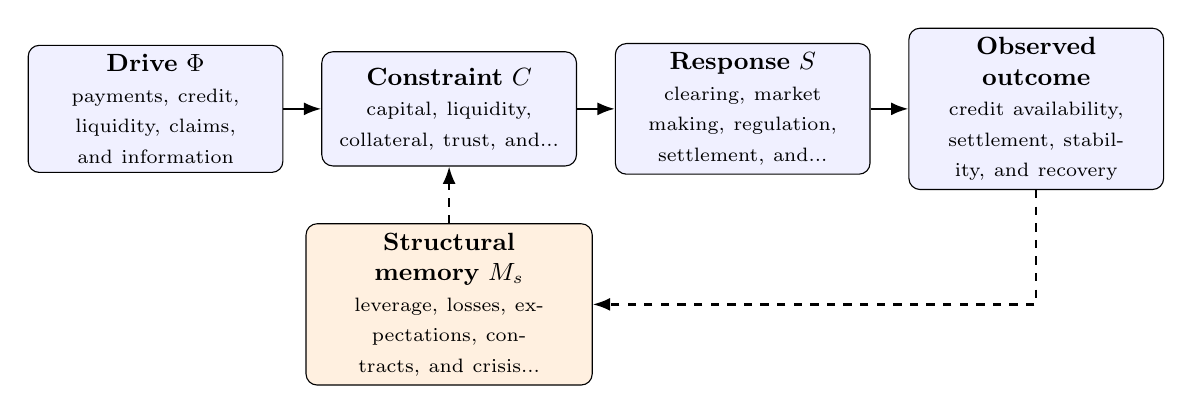
\begin{tikzpicture}[
    node distance=0.48cm,
    every node/.style={font=\small},
    box/.style={draw, rounded corners, align=center, minimum height=1.45cm, text width=3.0cm, fill=blue!6},
    memory/.style={draw, rounded corners, align=center, minimum height=1.25cm, text width=3.4cm, fill=orange!12},
    flow/.style={-{Latex[length=2.2mm]}, thick},
    feedback/.style={-{Latex[length=2.2mm]}, thick, dashed}
]
\node[box] (drive) {\textbf{Drive $\Phi$}\\\scriptsize payments, credit, liquidity, claims, and information};
\node[box, right=of drive] (constraint) {\textbf{Constraint $C$}\\\scriptsize capital, liquidity, collateral, trust, and...};
\node[box, right=of constraint] (response) {\textbf{Response $S$}\\\scriptsize clearing, market making, regulation, settlement, and...};
\node[box, right=of response] (outcome) {\textbf{Observed outcome}\\\scriptsize credit availability, settlement, stability, and recovery};
\node[memory, below=0.72cm of constraint] (memory) {\textbf{Structural memory $M_s$}\\\scriptsize leverage, losses, expectations, contracts, and crisis...};
\draw[flow] (drive) -- (constraint);
\draw[flow] (constraint) -- (response);
\draw[flow] (response) -- (outcome);
\draw[feedback] (outcome.south) |- (memory.east);
\draw[feedback] (memory.north) -- (constraint.south);
\end{tikzpicture}
\caption{Paper C-02 observable CDFD/AFL architecture for Financial Systems. Solid arrows give the proposed forward chain; dashed arrows make history-dependent feedback explicit.}
\label{fig:c02-architecture}
\end{figure}

\subsection{Paper-Specific Causal Hypothesis}

For this paper, the hypothesized causal sequence is specific. A change in
payments, credit, liquidity, claims, and information arrives faster than clearing, market making, regulation, settlement, and emergency support can compensate.
This raises or redistributes capital, liquidity, collateral, trust, and counterparty limits. If the load persists,
the retained state encoded by leverage, losses, expectations, contracts, and crisis history changes the next response, so a later event of equal
magnitude can produce a different trajectory in credit availability, settlement, stability, and recovery. The
scientific task is to estimate that sequence against the best ordinary model of
the domain, not merely to redescribe the outcome after it occurs.

\subsection{Cross-Scale Translation Without Mechanistic Erasure}

For the socioeconomic systems family, the cross-domain translation compares human and institutional throughput, unequal access to capacity, adaptive coordination, and historical path dependence. The variables are not morally neutral: aggregation can hide who receives flow, who bears constraint, and whose prior losses become persistent memory. \cite{BarabasiAlbert1999,WattsStrogatz1998,Holling1973,Shannon1948}
The required scale declaration for this paper is microseconds to decades; institutions to global finance. At short
scales, the key question is whether the incoming drive is transmitted,
buffered, or diverted. At intermediate scales, response changes effective
capacity and network exposure. At long scales, retained structure can alter the
state space itself. A result is genuinely cross-scale only when the aggregation
rule is stated and the same conclusion is not an artifact of averaging.

\subsection{Evidence Ladder and Discriminating Tests}

\begin{table}[htbp]
\centering
\small
\caption{Evidence ladder for Paper C-02. Each rung can fail independently.}
\begin{tabularx}{\textwidth}{|p{0.17\textwidth}|X|X|}
\hline
\textbf{Test} & \textbf{Design} & \textbf{Discriminating result} \\
\hline
Proxy audit & Measure balance sheets, transaction networks, spreads, defaults, and policy interventions and preregister how each record maps to $\Phi$, $C$, $S$, $M_s$, and $Y$. & The mapping fails if proxies are non-identifiable, circular, or change meaning across cases. \\
\hline
Load ramp & Apply or observe a liquidity or collateral shock across a connected financial network while estimating the dominant constraint and response time. & A threshold claim requires a reproducible nonlinear change and uncertainty bounds, not a visually chosen breakpoint. \\
\hline
Recovery and memory & Match present load across units with different histories, then compare recovery paths. & The memory claim requires history-dependent divergence after current conditions are controlled. \\
\hline
Model comparison & Compare the baseline domain model with and without the CDFD/AFL state variables using held-out data. & The paper's stated falsifier is: the mapping adds no value beyond established balance-sheet and network models. \\
\hline
\end{tabularx}
\end{table}

\subsection{Research Programme and Boundary Conditions}

The immediate research programme has four steps. First, construct a documented
dataset from balance sheets, transaction networks, spreads, defaults, and policy interventions and retain raw units before normalization.
Second, fit a baseline domain model and report its calibration and out-of-sample
error. Third, add the smallest identifiable CDFD/AFL state extension and test
whether it improves prediction of credit availability, settlement, stability, and recovery. Fourth, repeat the
analysis across the declared scale range and publish negative cases as part of
the cross-domain translation audit.

% END PART IV MAJOR CROSS-DOMAIN UPGRADE

\section{Conclusion}
Financial markets are non-linear thermodynamic transport networks. Debt acts as a topological memory lock, and capital acts as a driving flux. By modeling economies through CDFD, policymakers can identify structural instabilities before they result in catastrophic topological phase shifts.
\section*{Conflict of Interest} The author declares no conflict of interest.
\section*{Data Availability}
Part-specific runtime diagnostics are under each Part's \path{outputs/} directory.

Release-wide code: \path{Part_E_Synthesis/supplementary/}.

Generated summaries: \path{Part_E_Synthesis/outputs/}.

Figures: \path{Part_E_Synthesis/figures/}.


\section{Reference Layer}
\bibliographystyle{plain}
\bibliography{universal_afl_references}
\end{document}
